\documentclass[10pt,a4paper]{article}
\usepackage[latin1]{inputenc}
\usepackage{amsmath}
\usepackage{microtype}
\usepackage[none]{hyphenat}
\usepackage{verbatim}
\usepackage{amsfonts}
\usepackage{amssymb}
\usepackage{enumitem}
\renewcommand{\familydefault}{\sfdefault}
\usepackage{mathpazo}
\renewcommand{\rmdefault}{put}
\usepackage{enumitem}
\usepackage[dvipsnames,svgnames]{xcolor}
\usepackage{tkz-euclide}
\usetkzobj{all}
\usepackage{graphicx}
\usepackage{fancyhdr}
\usepackage{tikz} 	
\usepackage{adjustbox}
\usepackage{pgfplots}
\usepackage{multicol}
\usepackage{lipsum}
\usepackage[left=0.7cm,right=1cm,top=1cm,bottom=1.5cm]{geometry}
\usepackage{cancel} \usepackage{xcolor}
\usepackage{tcolorbox}
\usetikzlibrary{decorations.pathmorphing,patterns}
\usetikzlibrary{decorations.pathreplacing,calc}
 \newcommand\coret[2][red]{\renewcommand\CancelColor{\color{#1}}\cancel{#2}}
\SetLabelAlign{Center}{\hfil\makebox[1.0em]{#1}\hfil}

%%_------= solusi


% Set this =0 to hide, =1 to show

% Set this =0 to hide, =1 to show
\newtcolorbox{mybox}[1][] { colframe = blue!10, colback = blue!3,boxsep=0pt,left=0.2em, coltitle = blue!20!black, title = \textbf{}, #1, } 

%---------- kunci (jika 1 ) muncul
\def\tampilkunci{1}
\newcommand{\hide}[1]{\ifnum\tampilkunci=1
%
\begin{mybox}
 #1
\end{mybox}
%
\vspace{\baselineskip}\fi\ifnum\tampilkunci=0
%
%\vspace{2cm}
%
\fi}



\newcommand*\cicled[1]{\tikz[baseline=(char.base)]{\node[white, shape=circle, fill=red!80,draw,inner sep=0.5pt](char){#1};}}

\newcommand*\kunci[1]{\ifnum\tampilkunci=1
%
\tikz[baseline=(char.base)]{\node[red, shape=circle,draw,inner sep=0.5pt,xshift=2pt](char){#1};}\stepcounter{enumii}
\fi\ifnum\tampilkunci=0
%
\hspace{3pt}#1\stepcounter{enumii}
%
\fi}

\newcommand*\silang[1]{\tikz[baseline=(char.base)]{
\draw[red,thick](-0.2,-0.20)--(0.2,0.2);
\draw[red,thick](-0.2,0.20)--(0.2,-0.2);
\node[black](char){#1};
}}

\newcommand*\centang[1]{\tikz[baseline=(char.base)]{
\draw[red, very thick](-0.2,0.1)--(-0.1,0)--(0.2,0.3);
\node(char){#1};
}}

\newcommand*\merah[1]{
\textcolor{red}{#1}}
\newcommand*\pilgan[1]{
\begin{enumerate}[label=\Alph*., itemsep=0pt,topsep=0pt,leftmargin=*,align=Center] #1 
\end{enumerate}}
\newcommand*\pernyataan[1]{
\begin{enumerate}[label=(\arabic*), itemsep=0pt,topsep=0pt,leftmargin=*] #1 
\end{enumerate}}
\pagestyle{fancy}
\renewcommand{\headrulewidth}{0pt}
\rfoot{\tiny{arifstwan}}
\newcommand{\pilgani}[1]{                            \vspace{-0.3cm}\begin{multicols}{2}
 \begin{enumerate}[label=\Alph*., itemsep=0pt,topsep=0pt,leftmargin=*,align=Center]#1                     \end{enumerate}
 \phantom{ini cuma sapi, wedus, dan ayam}
 \end{multicols}}


\begin{document}


 \textbf{Mandiri-Momentum} \phantom{ini nama siswa yang aaamengerjakan soal kuis ini }  

No callculator allowed !  
\begin{multicols*}{2}
\begin{enumerate}
% no26 ---------------------------------------------------------
\item[7] Pembahasan jawaban
\hide{
\setlength{\tabcolsep}{0.1\tabcolsep}
diketahui :

\begin{tabular}{p{0.5cm} p{1mm} p{2cm} p{1cm} p{0.5cm} p{2cm} }
$h$ &: &80m  & & &\\
$e$ &: &0,2 & & & 
\end{tabular}

Ditanya: $v'=$ ?

Dijawab:
\begin{align*}
e&=\sqrt{\frac{h'}{h}}=\sqrt{\frac{h'}{80}}\\
0,2 &= \sqrt{\frac{h'}{80}}\\
\frac{4}{100} &=\frac{h'}{80}\\
h' &= 3,2
\end{align*}
 kecepatan agar sampai ketinggian 3,2 adalah
\begin{align*}
v& =\sqrt{2gh'}=\sqrt{2.10.3,2}=8\text{ m/s}
\end{align*}

}
\item[13] Pembahasan Jawaban
\hide{
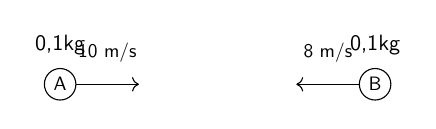
\begin{tikzpicture}
\foreach \x /\y/\z in {0/A/{0,1kg},4/B/{0,1kg}} {
\draw (\x,0) circle (0.2) node[scale=0.7]{\y};
\node at (\x,0.5) [scale=0.8]{\z};}
\draw[->] (0.2,0)--node[midway, yshift=0.4cm,scale=0.7]{10 m/s}(1,0);
\draw[->] (3.8,0)--node[midway, yshift=0.4cm,scale=0.7]{8 m/s}(3,0);
\end{tikzpicture}

Diketahui:

\begin{tabular}{p{0.5cm} p{1mm} p{2cm} p{1cm} p{0.5cm} p{2cm} }
$m_A$ &= &0.1 kg  & & &\\
$m_B$ &= &0.1 kg  & & &\\
$v_A$ &= &10 m/s  & & &\\
$v_B$ &= &-8 m/s  & & &\\
$e$ &= &1  & & &\\
\end{tabular}

Ditanya : $v_A'$ atau $v_1'$ dan $EK_A'$ ?

Jawab:

Karena lenting sempurna maka berlaku
\begin{align*}
e &= \frac{-(v_2'-v_1')}{v_2-v_1}\\
1 &= \frac{-v_2'+v_1'}{-8-(10)}\\
1 &= \frac{-(v_2'-v_1')}{-18}\\
\coret{-}18 &= \coret{-}(v_2'-v_1')\\
18 &= v_2' -v_1'
\end{align*}
Berlaku pula persamaan kekekalan momentum, massa sama
\begin{align*}
\Sigma p &= \Sigma p\\
\coret{m_A}v_1 + \coret{m_B}v_2 &= \coret{m_A}v_1' + \coret{m_B}v_2' \\
10-8 &= v_1' + v_2'\\
2 &= v_1' + v_2'
\end{align*}}
\hide{
Kemudian proses eliminasi sehingga 
\begin{align*}
18 &= v_2' -v_1'\\
2 &= v_2' + v_1'\\
\text{----}&\text{----------------(-)}\\
16 &=-2v_1'\\
v_1' &= -8 \text{ m/s}
\end{align*}
energi Kinetiknya $\frac{1}{2}mv^2=3,2$ J

Jika mereka \textbf{MASSA SAMA dan LENTING SEMPURNA} maka hanya bertukar kecepatan. Sehingga $v_1'=v_2=-8$ dengan arah ke kiri. }
\item[17] Pembahasan Jawaban
\hide{ 
Diketahui:

\begin{tabular}{p{0.5cm} p{1mm} p{2cm} p{1cm} p{0.5cm} p{2cm} }
$m_A$ &= &$m$  & & &\\
$m_B$ &= &$m$  & & &\\
$v_A$ &= &10 m/s  & & &\\
$v_B$ &= &-20 m/s  & & &\\
$e$ &= &1  & & &\\
\end{tabular}

Ditanya : $v_A'$ dan  $v_B'$  ?

Jawab : 

Sesuai soal yang di atas, karena massa sama dan lenting sempurna maka bertukar kecepatan. Kecepatan akhir A $_A'=-20$ m/s dan kecepatan  akhir B $v_B'=10$ m/s. Jawabannya B
}


\item[22] Pembahasan Jawaban
\hide{

Diketahui:

\begin{tabular}{p{0.5cm} p{1mm} p{2cm} p{1cm} p{0.5cm} p{2cm} }
$m_A$ &= & 2 kg  & & &\\
$m_B$ &= & 1 kg  & & &\\
$v_A$ &= & 3 m/s  & & &\\
$v_B$ &= & 0 m/s  & & &\\
$e$ &= &1  & & &\\
\end{tabular}

Ditanya : $v_A'$ dan $v_B'$ ?

Jawab:

Karena lenting sempurna maka berlaku
\begin{align*}
e &= \frac{-(v_2'-v_1')}{v_2-v_1}\\
1 &= \frac{-v_2'+v_1'}{0-(3)}\\
1 &= \frac{-(v_2'-v_1')}{-3}\\
\coret{-}3 &= \coret{-}(v_2'-v_1')\\
3 &= v_2' -v_1'
\end{align*}}
\hide{
Berlaku pula persamaan kekekalan momentum, 
\begin{align*}
\Sigma p &= \Sigma p\\
{m_A}v_1 + {m_B}v_2 &= {m_A}v_1' + {m_B}v_2' \\
2.3+1.0 &= 2v_1' +1v_2'\\
6 &= 2v_1' + v_2'
\end{align*}
Kemudian proses eliminasi sehingga 
\begin{align*}
3 &= v_2' -v_1'\\
6 &= v_2' + 2v_1'\\
\text{----}&\text{----------------(-)}\\
-3 &=-3v_1'\\
v_1' &= 1 \text{ m/s}\\
v_2' &= 4 \text{ m/s}
\end{align*}
}
\item[25] Pembahasana Jawaban
\hide{

Diketahui:

\begin{tabular}{p{0.5cm} p{1mm} p{2cm} p{1cm} p{0.5cm} p{2cm} }
$m_A$ &= & 3 kg  & & &\\
$m_B$ &= & 2 kg  & & &\\
$v_A$ &= & 5 m/s  & & &\\
$v_B$ &= & -2,5 m/s  & & &\\
$e$ &= &1  & & &\\
\end{tabular}

Ditanya : $v_A'$  ?

Jawab:

Karena lenting sempurna maka berlaku
\begin{align*}
e &= \frac{-(v_2'-v_1')}{v_2-v_1}\\
1 &= \frac{-v_2'+v_1'}{-2,5-(5)}\\
1 &= \frac{-(v_2'-v_1')}{-7,5}\\
\coret{-}7,5 &= \coret{-}(v_2'-v_1')\\
7.5 &= v_2' -v_1'
\end{align*}
Berlaku pula persamaan kekekalan momentum, 
\begin{align*}
\Sigma p &= \Sigma p\\
{m_A}v_1 + {m_B}v_2 &= {m_A}v_1' + {m_B}v_2' \\
3(5)+2.(-2,5) &= 3v_1' +2v_2'\\
10 &= 3v_1' + 2v_2'
\end{align*}
Kemudian proses eliminasi sehingga 
\begin{align*}
7.5 &= v_2' -v_1'\\
10 &= 3v_1' + 2v_2'\\
\text{persamaan 1 dikali}&\text{ 2 dulu}\\
15 &=2v_2'-2v_1'\\
10 &= 3v_1'+2v_2'\\
\text{----}&\text{--------------(-)}\\
5 &= -5v_1'\\
v_1'&= -1 \text{ m/s}
\end{align*}
}


\item[27] Pembahasan Jawaban
\hide{
diketahui :

\begin{tabular}{p{0.5cm} p{1mm} p{2cm} p{1cm} p{0.5cm} p{2cm} }
$h$ &: &1.5 m  & & &\\
$e$ &: &0,4 & & & 
\end{tabular}

Ditanya: $v'=$ ?

Dijawab:

Gunakan persamaan restitusi $e$ 
$$ e = \sqrt{\frac{h'}{h}}=\frac{-(v_2'-v_1')}{v_2-v_1}$$
\begin{align*}
e&=\sqrt{\frac{h'}{h}}=\sqrt{\frac{h'}{1.5}}\\
0,4 &= \sqrt{\frac{h'}{1.5}}\\
\frac{16}{100} &=\frac{h'}{1.5}\\
h' &= 0,24 \text { m} 
\end{align*}
} 

\item[30] Pembahasan Jawaban
\hide{
diketahui :

\begin{tabular}{p{0.5cm} p{1mm} p{2cm} p{1cm} p{0.5cm} p{2cm} }
$m_A$ &: & 3 kg  & & &\\
$m_B$ &: & 2 kg  & & &\\
$v_A$ &: & 2 m/s  & & &\\
$v_B$ &: & -3 m/s  & & &\\
\end{tabular}

Ditanya: $v_B'=$ ?

Dijawab:

Setelah dihitung menggunakan cara di atas maka kecepatan akhir B  $v_B'$= 3 m/s

}

\item[31] Pembahasan Jawaban
\hide{
Massa sama dan lenting sempurna sehingga bertukar kecepatan

Awal : $v_A$ = 15 m/s (kanan), $v_B$ = - 25 m/s (kiri)

Akhir : $v_A'$ = -25 m/s (kiri) , $v_B'$ = 15 m/s(kanan)

Jadi kecepatannya adalah 25 m/s dan 15 m/s berlawanan gerak awal


}

\item[35] Pembahasan Jawaban
\hide{
Sebelum menjawab perhatikan soalnya, kecepatan bola A adalah 5 m/s. Setelah 2 detik menempuh jarak 14 m. Padalah secara logika 2 detik hanya 10 m. Berarti terjadi GLBB, harus dicari percepatannya $a$

\begin{align*}
s &=v_o.t + \frac{1}{2}at^2\\
14 &=5.2 + \frac{1}{2}a(2)^2\\
a &= 2
\end{align*}

Saat mereka bertumbukan kecepatan A adalah
\begin{align*}
v_t &= v_o + a.t = 5 + 2.2 = 9 \text{ m/s}
\end{align*}

Mereka bertumbukan tidak lenting sama sekali. Artinya mereka bersatu setelah tmbukan
\begin{align*}
\Sigma p &= \Sigma p'\\
m_A.(9) + m_B.(-15) &= (m_A+ m_B)v'\\
m(9) + m(-15) &= (m+m)v'\\
m(-6) &= 2m v'\\
v'&= -3 \text{ m/s}
\end{align*}
}







\end{enumerate}
\end{multicols*} \end{document} 

